\documentclass[12pt]{beamer}

\usetheme{Oxygen}
\usepackage{thumbpdf}
\usepackage{wasysym}
\usepackage{ucs}
\usepackage[utf8]{inputenc}
\usepackage{pgf,pgfarrows,pgfnodes,pgfautomata,pgfheaps,pgfshade}
\usepackage{verbatim}
\usepackage{graphicx}

\pdfinfo
{
  /Title       (Introdução ao Docker)
  /Creator     (Thiago Almeida)
  /Author      (Thiago Almeida)
}


\title{Introdução ao Docker}
\subtitle{O que é e porque devo utilizar?}
\date{\today}

\begin{document}
\author{Thiago Almeida
    	\href{mailto:thiagoalmeida@ufpa.br}{thiagoalmeida@ufpa.br}}

\frame{\titlepage}

\newcommand<>{\highlighton}[1]{%
  \alt#2{\structure{#1}}{{#1}}
}

\newcommand{\icon}[1]{\pgfimage[height=1em]{#1}}



\newcommand{\putlink}[1]{%
   \pgfsetlinewidth{1.4pt}%
   \pgfsetendarrow{\pgfarrowtriangle{4pt}}%
   \pgfline{\pgfxy(1,1)}{\pgfxy(#1,1)}
}
%%%%%%%%%%%%%%%%%%%%%%%%%%%%%%%%%%%%%%%%%
%%%%%%%%%% Content starts here %%%%%%%%%%
%%%%%%%%%%%%%%%%%%%%%%%%%%%%%%%%%%%%%%%%%



\section{Apresentação}
\begin{frame}
  \frametitle{Pré requisitos e Objetivos}
  \begin{block}{Docker}
  \begin{itemize}
		\item Nenhuma experiência anterior com \emph{Docker} será necessária.
  \end{itemize}
  \end{block}

	\begin{block}{\emph{LINUX}}
  \begin{itemize}
		\item Familiariadade com alguma distribuição \emph{Linux}
		\item Familiariadade com terminal e linhas de comando.
  \end{itemize}
  \end{block}

  \begin{block}{Objetivos}
  \begin{itemize}
		\item Entender a a estrutura da plataforma \emph{Docker}.
		\item Conhecer os componentes da plataforma \emph{Docker}.
			\begin{itemize}
				\item Imagens
				\item Contêineres
				\item Repositórios
			\end{itemize}
  \end{itemize}
  \end{block}
\end{frame}
\section{Introdução}
\begin{frame}
  \frametitle{Agenda}
  \framesubtitle{Tópicos abordados}
  \begin{block}{Principais pontos}
		\begin{itemize}
			\item O que é Docker?
			\pause
			\item Contêineres vs Máquinas Virtuais
			\pause
			\item Visualização sobre a plataforma Docker
			\pause
				\begin{itemize}
					\item Docker Engine
					\pause
					\item Imagens
					\pause
					\item Contêineres
					\pause
					\item Registro
					\pause
					\item Repositórios
					\pause
				\end{itemize}
			\item Introdução às Imagens
			\pause
			\item Iniciando com contêineres
  			\end{itemize}
  \end{block}
\end{frame}
\begin{frame}
  \frametitle{O que é Docker?}
  \begin{block}{Definição}
					Docker é uma plataforma para desenvolvimento, envio e execução de
					aplicações utilizando virtualização baseada em contêiner.
					A plataforma \emph{Docker} é composta por algumas ferramentas e
					produtos, são eles:
  \begin{itemize}
		\item \emph{Docker Engine}
		\pause
		\item \emph{Docker Hub}
		\pause
		\item \emph{Docker Machine}
		\pause
		\item \emph{Docker Swarm}
		\pause
		\item \emph{Docker Compose}
  \end{itemize}
  \end{block}
\end{frame}
\begin{frame}
  \frametitle{Contêineres vs Máquinas Virtuais}
  \framesubtitle{Um pouco de história}
  \begin{block}{Servidores reais}
		Antigamente nós utilizávamos um servidor para uma única aplicação.
		\begin{figure}[!h]
			\centering
			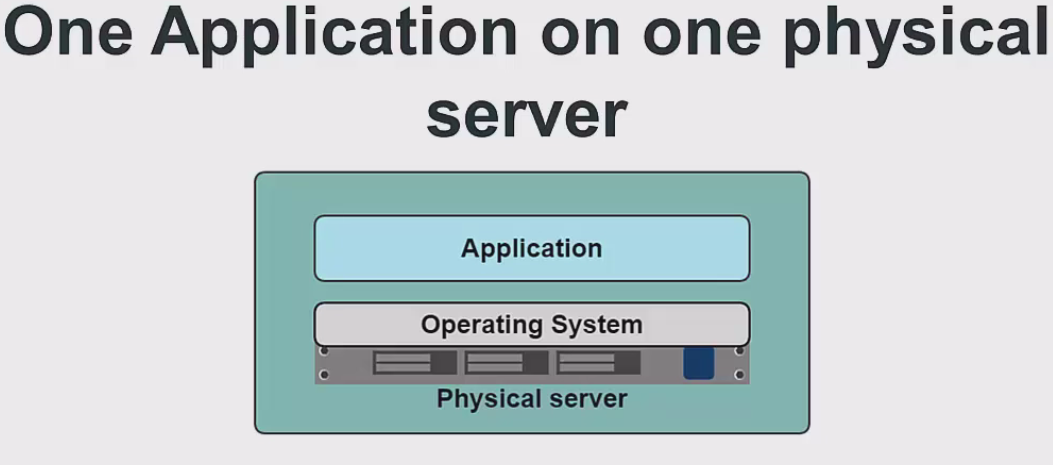
\includegraphics[width=0.6\paperwidth]{physicalserver}
		\end{figure}
  \end{block}
\end{frame}
\begin{frame}
  \frametitle{Contêineres vs Máquinas Virtuais}
  \framesubtitle{Um pouco de história}
  \begin{block}{Problemas que isso causava}
	\begin{itemize}
		\item Gastava muito tempo no \emph{deploy}
		\pause
		\item Alto custo
		\pause
		\item Desperdício de recursos
		\pause
		\item Difícil para escalar
		\pause
		\item Difícil para migrar
		\pause
		\item Dependência do fabricante
	\end{itemize}
  \end{block}
\end{frame}
\begin{frame}
  \frametitle{Contêineres vs Máquinas Virtuais}
  \framesubtitle{Um pouco de história}
	\begin{block}{Virtualização baseada em \emph{Hypervisor}}
	\begin{itemize}
		\item Um servidor físico pode conter várias aplicações
		\pause
		\item Cada aplicação roda em uma máquina virtual (\emph{VM})
		\begin{figure}[!h]
			\centering
			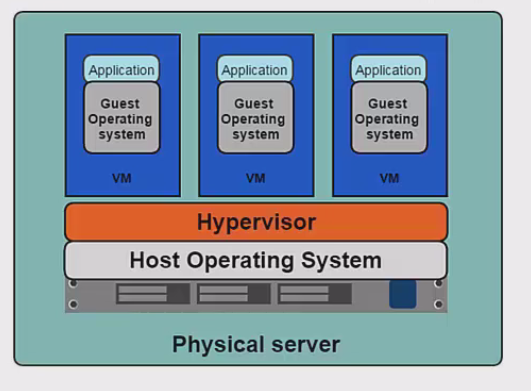
\includegraphics[width=0.6\paperwidth]{hypervisor}
		\end{figure}
	\end{itemize}
  \end{block}
\end{frame}
\begin{frame}
  \frametitle{Contêineres vs Máquinas Virtuais}
  \framesubtitle{Um pouco de história}
	\begin{block}{Vantagens da máquina virtual}
	\begin{itemize}
		\item Melhor aproveitamento dos recursos
		\pause
		\item Um servidor físico dividido em várias máquinas virtuais
		\pause
		\item Fácil de escalar
		\pause
	\end{itemize}
  \end{block}
	\begin{block}{Limitações da máquina virtual}
		\begin{itemize}
			\item Cada máquina virtual requer:
			\pause
				\begin{itemize}
				\item CPU alocada
				\pause
				\item Armazenamento
				\pause
				\item Memória RAM
				\pause
				\item Um sistema operacional inteiro
			\end{itemize}
			\pause
			\item Quanto mais \emph{VMs} você roda, mais recursos você precisa
			\pause
			\item Um sistema operacional num \emph{guest} é um desperdício
		\end{itemize}
	\end{block}
\end{frame}
\begin{frame}
  \frametitle{Contêineres vs Máquinas Virtuais}
  \framesubtitle{Introdução aos contêineres}
	\begin{block}{O que são?}
					Virtualização baseada em contêiner usa o \emph{kernel} do sistema
					operacional do \emph{host} para executar múltiplas instâncias
	\end{block}
	\begin{block}{}
	\begin{itemize}
		\item Cada \emph{guest} é chamado de \textbf{contêiner}
		\pause
		\item Cada contêiner possui:
		\pause
			\begin{itemize}
				\item Sistema de arquivos raiz
				\pause
				\item Processos
				\pause
				\item Memória
				\pause
				\item Dispositivos
				\pause
				\item Pilha de rede
			\end{itemize}
	\end{itemize}
	\end{block}
\end{frame}
\begin{frame}
  \frametitle{Contêineres vs Máquinas Virtuais}
  \framesubtitle{Contêiner}
	\begin{block}{Visualizando um contêiner}
		\begin{figure}[!h]
			\centering
			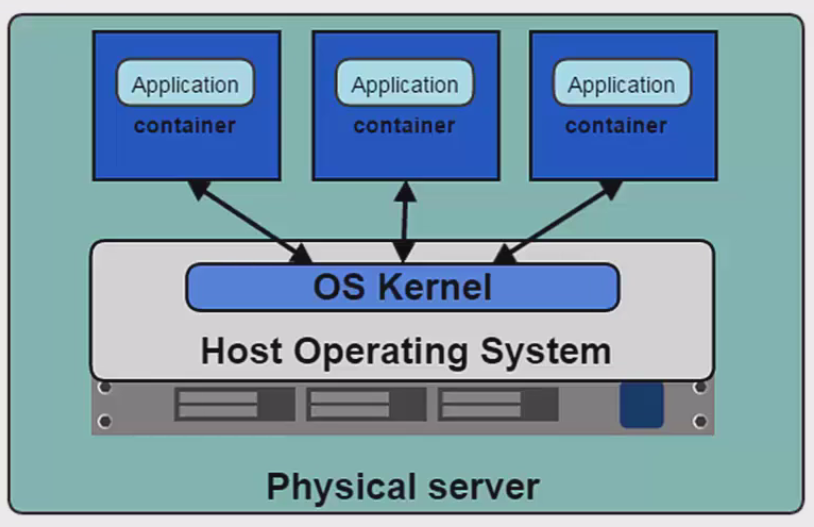
\includegraphics[width=0.6\paperwidth]{container}
		\end{figure}
	\end{block}
\end{frame}
\begin{frame}
  \frametitle{Contêineres vs Máquinas Virtuais}
  \framesubtitle{Contêiner vs VM}
	\begin{block}{Vantagens do contêiner}
		\begin{itemize}
			\item Contêiner é mais leve
			\pause
			\item Não precisa instalar um SO inteiro
			\pause
			\item Requer menos \emph{CPU, RAM} e armazenamento 
			\pause
			\item Um servidor pode rodar mais contêineres do que \emph{VMs}
			\pause
			\item Maior portabilidade
		\end{itemize}
	\end{block}
\end{frame}
\begin{frame}
  \frametitle{Contêineres vs Máquinas Virtuais}
  \framesubtitle{Visualizando as diferenças}
	\begin{block}{}
		\begin{figure}[!h]
			\centering
			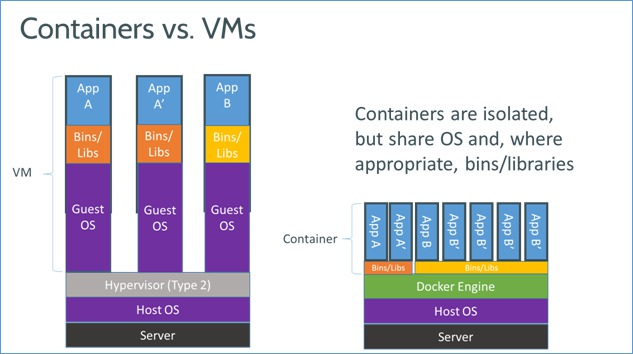
\includegraphics[width=0.6\paperwidth]{vmvscontainer}
		\end{figure}
	\end{block}
\end{frame}
\section{Docker, conceitos e termos}
\begin{frame}
  \frametitle{Docker Engine}
	\begin{block}{O que é?}
		\begin{itemize}
			\item \emph{Docker Engine} é o programa que possibilita os
										contêineres serem feitos, enviados e executados.
			\pause
			\item \emph{Docker Engine} utiliza \emph{namespaces e cgroups} do
							\emph{Kernel Linux}.
			\pause
			\item \emph{Namespaces} nos permitem isolar os contêineres nos seus
							próprios ambientes.
			\pause
		\end{itemize}
	\end{block}
\end{frame}
\begin{frame}
  \frametitle{Composição do Docker Engine}
	\begin{block}{Docker Client e Daemon}
		\begin{itemize}
			\item Possui a arquitetura Cliente/Servidor
			\pause
			\item O cliente pega as entradas do usuário e às envia pro \emph{Daemon}
			\pause
			\item O \emph{Daemon} monta, executa e distribui os contêineres.
			\pause
			\item Cliente e \emph{Daemon} podem rodar no mesmo \emph{host} ou em
							\emph{hosts} diferentes.
			\pause
		\end{itemize}
	\end{block}
\end{frame}
\begin{frame}
  \frametitle{Docker Contêineres e Imagens}
	\begin{block}{Imagens}
		\begin{itemize}
			\item \emph{Template} somente leitura utilizado para criar contêineres
			\pause
			\item Feita por você mesmo ou outro usuários Docker
			\pause
			\item Armazenada no \emph{Docker Hub} ou no seu \emph{Registro local}
			\pause
		\end{itemize}
	\end{block}
	\begin{block}{Contêineres}
		\begin{itemize}
			\item Plataforma isolada para a aplicação
			\pause
			\item Contém tudo que precisa para executar a aplicação
			\pause
			\item Baseado em uma ou mais imagens
			\pause
		\end{itemize}
	\end{block}
\end{frame}
\begin{frame}
  \frametitle{Docker Registro e Repositório}
	\begin{block}{Registro}
		\begin{itemize}
			\item Registro é onde nós armazenamos as nossas imagens.
			\pause
			\item Podemos ter o nosso próprio Registro ou utilizar Registros públicos
							como o \emph{Docker Hub}
		\end{itemize}
	\end{block}
	\begin{block}{Repositórios}
		\begin{itemize}
			\item Dentro do Registro nós temos os Repositórios
		\end{itemize}
	\end{block}
\end{frame}
\end{document}
